\section{DevOps and Deployment Strategy}

Getting our platform from development to production required setting up a solid DevOps pipeline. We needed something that could handle both our local development needs and production deployment without breaking anything along the way. The setup we built uses containerization for consistency and automated pipelines for reliability.

\subsection{EasyPanel Infrastructure}

We have used EasyPanel running on a dedicated Mac Studio server. This self-hosted approach gives us complete control over our deployment process and keeps costs reasonable and the Mac Studio provides plenty of power for our needs. The setup handles automatic SSL certificates through Let's Encrypt and Traefik \cite{traefik2025docker}, container orchestration, and provides a clean interface for managing deployments.

\begin{figure}[H]
    \centering
    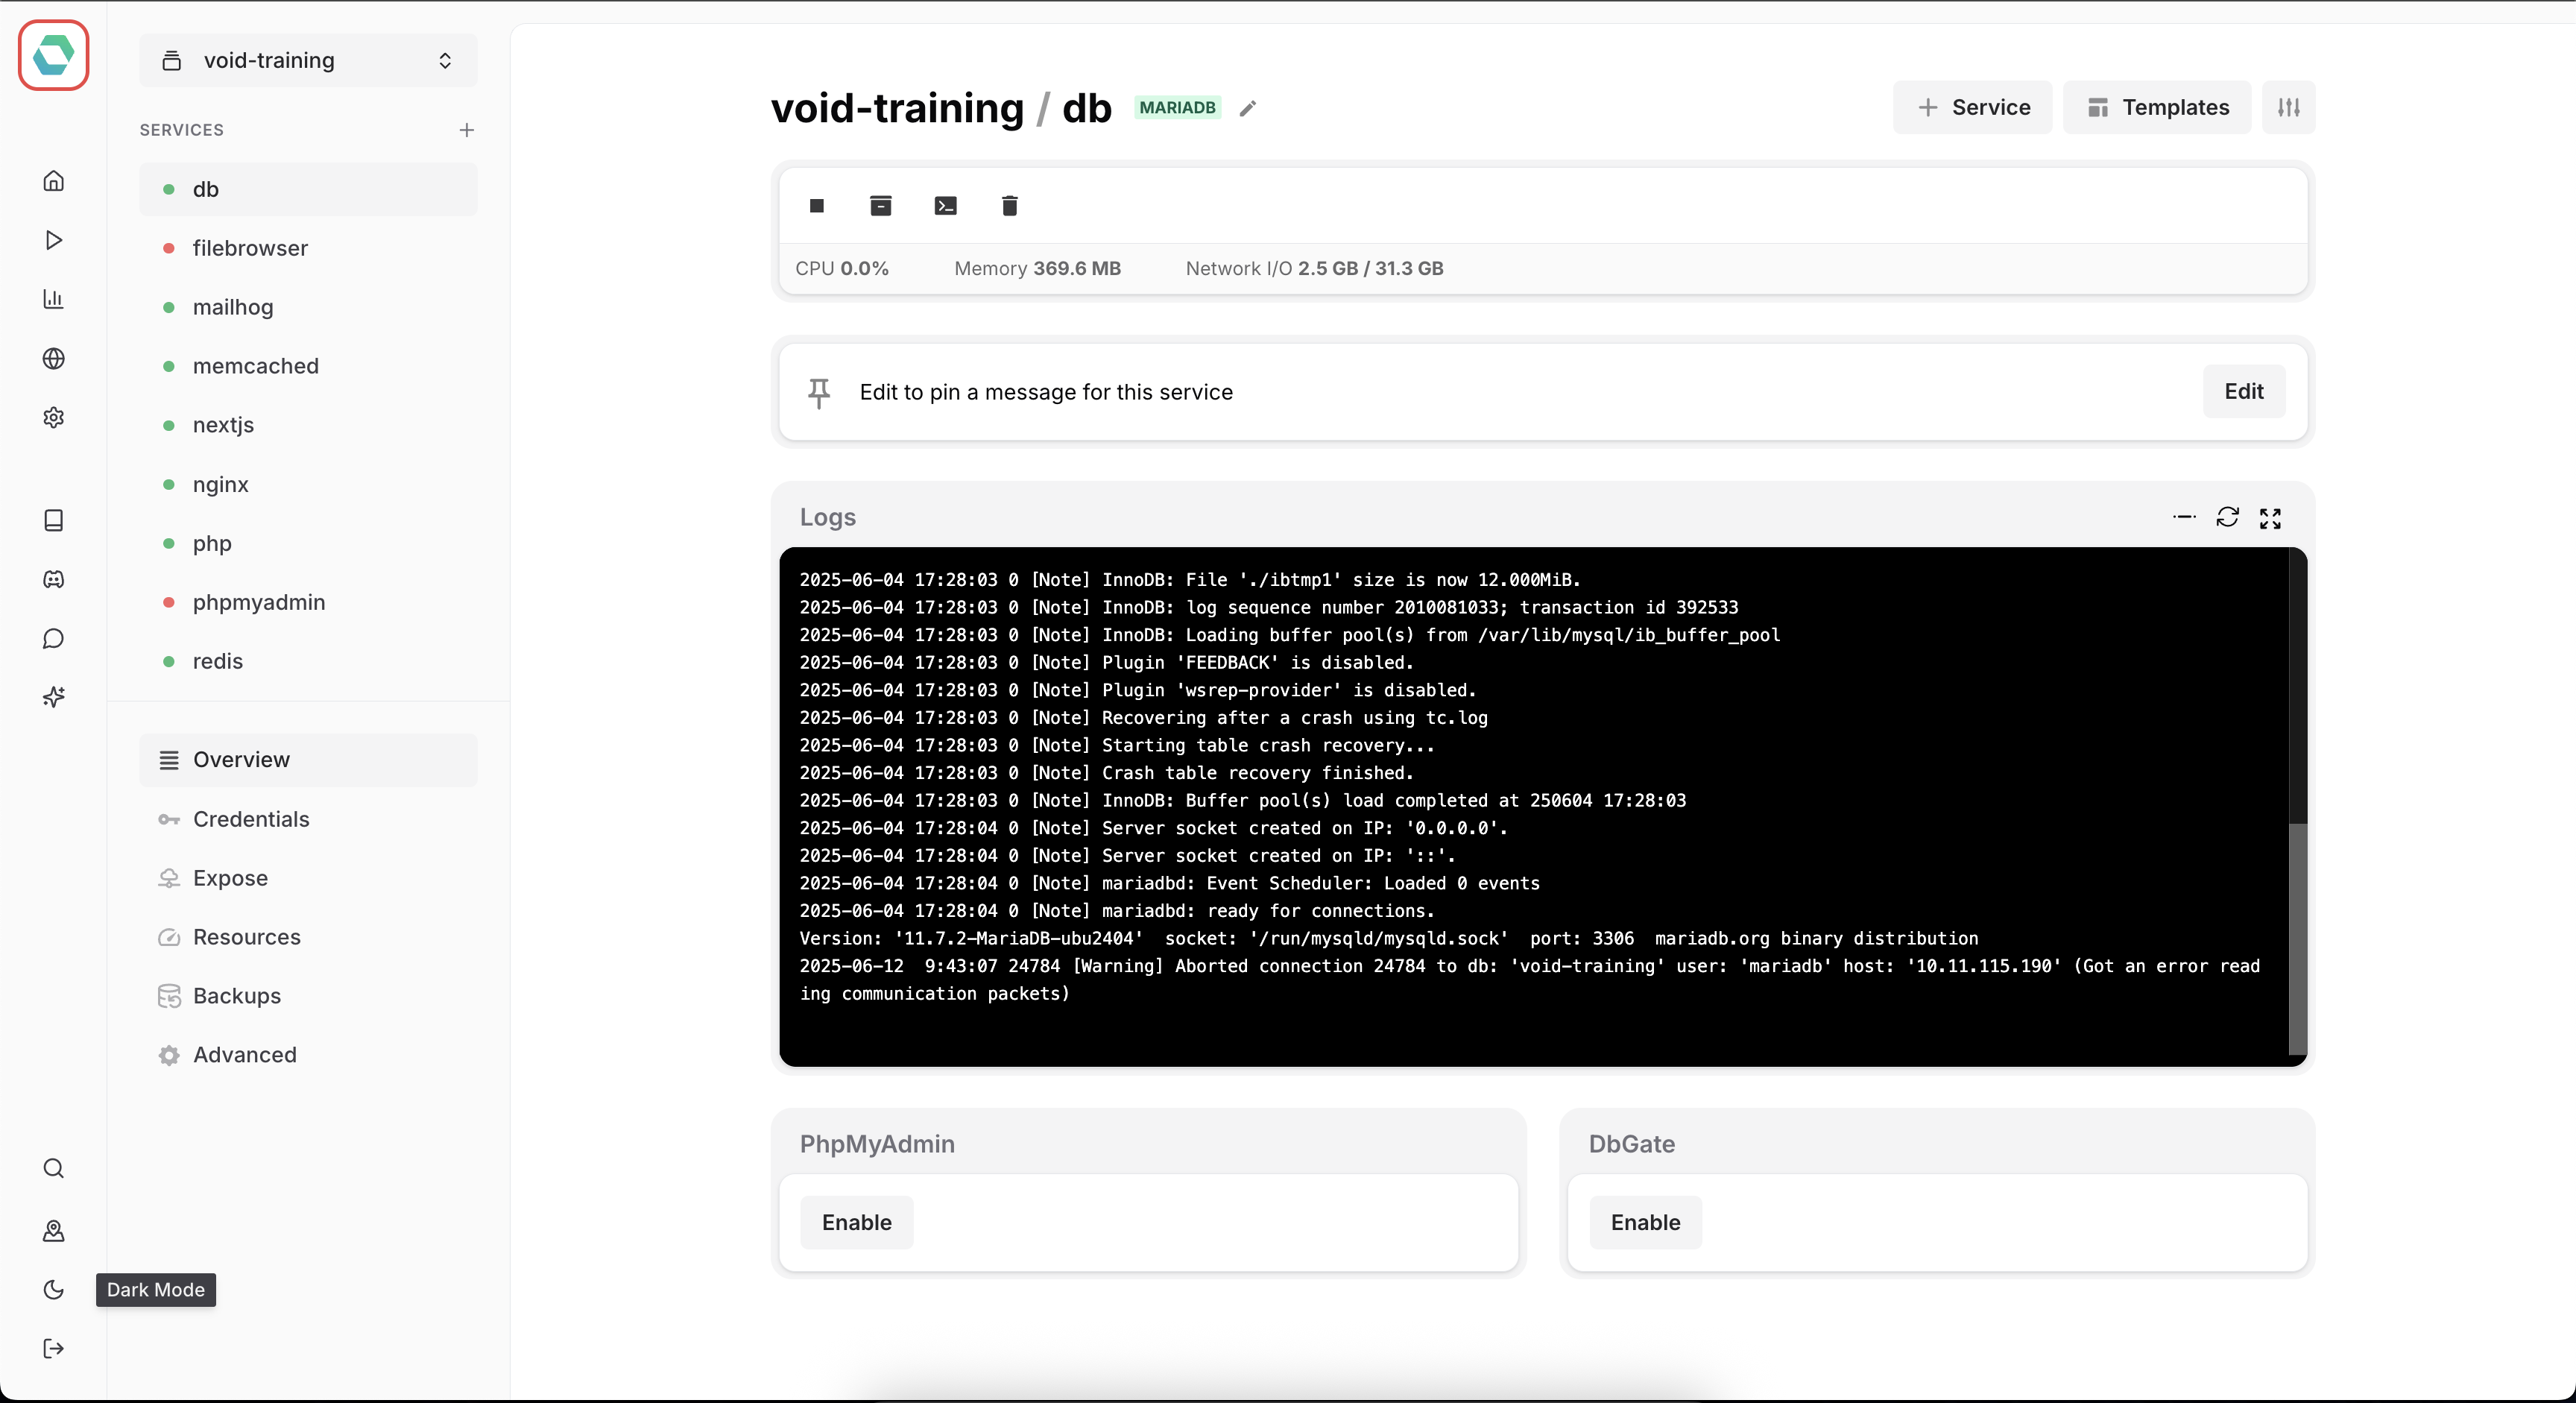
\includegraphics[width=0.95\textwidth]{images/Screenshot-easypanel.png}
    \caption{EasyPanel Production Environment}
    \label{fig:easypanel_env}
\end{figure}

\subsection{Continuous Integration and Deployment Pipeline (CI/CD)}

Besides that, we have built a CI/CD pipeline that automates everything from code changes to production deployment. We have used a tag-based deployment system that automatically builds and deploys our code when we created release tags. Here's how it works:

\begin{enumerate}
    \item We commit code changes to feature branches
    \item After code review, changes get merged to main
    \item When ready for release, we create a tag (like v1.2.3)
    \item Bitbucket webhook triggers a DockerHub build automatically
    \item DockerHub builds and tags container images (build fails if ESLint or Prettier tests don't pass)
    \item EasyPanel pulls the updated images by tag
    \item Rolling deployment happens automatically
\end{enumerate}

Below are the DockerHub build processes for the frontend and backend:

\begin{figure}[H]
    \centering
    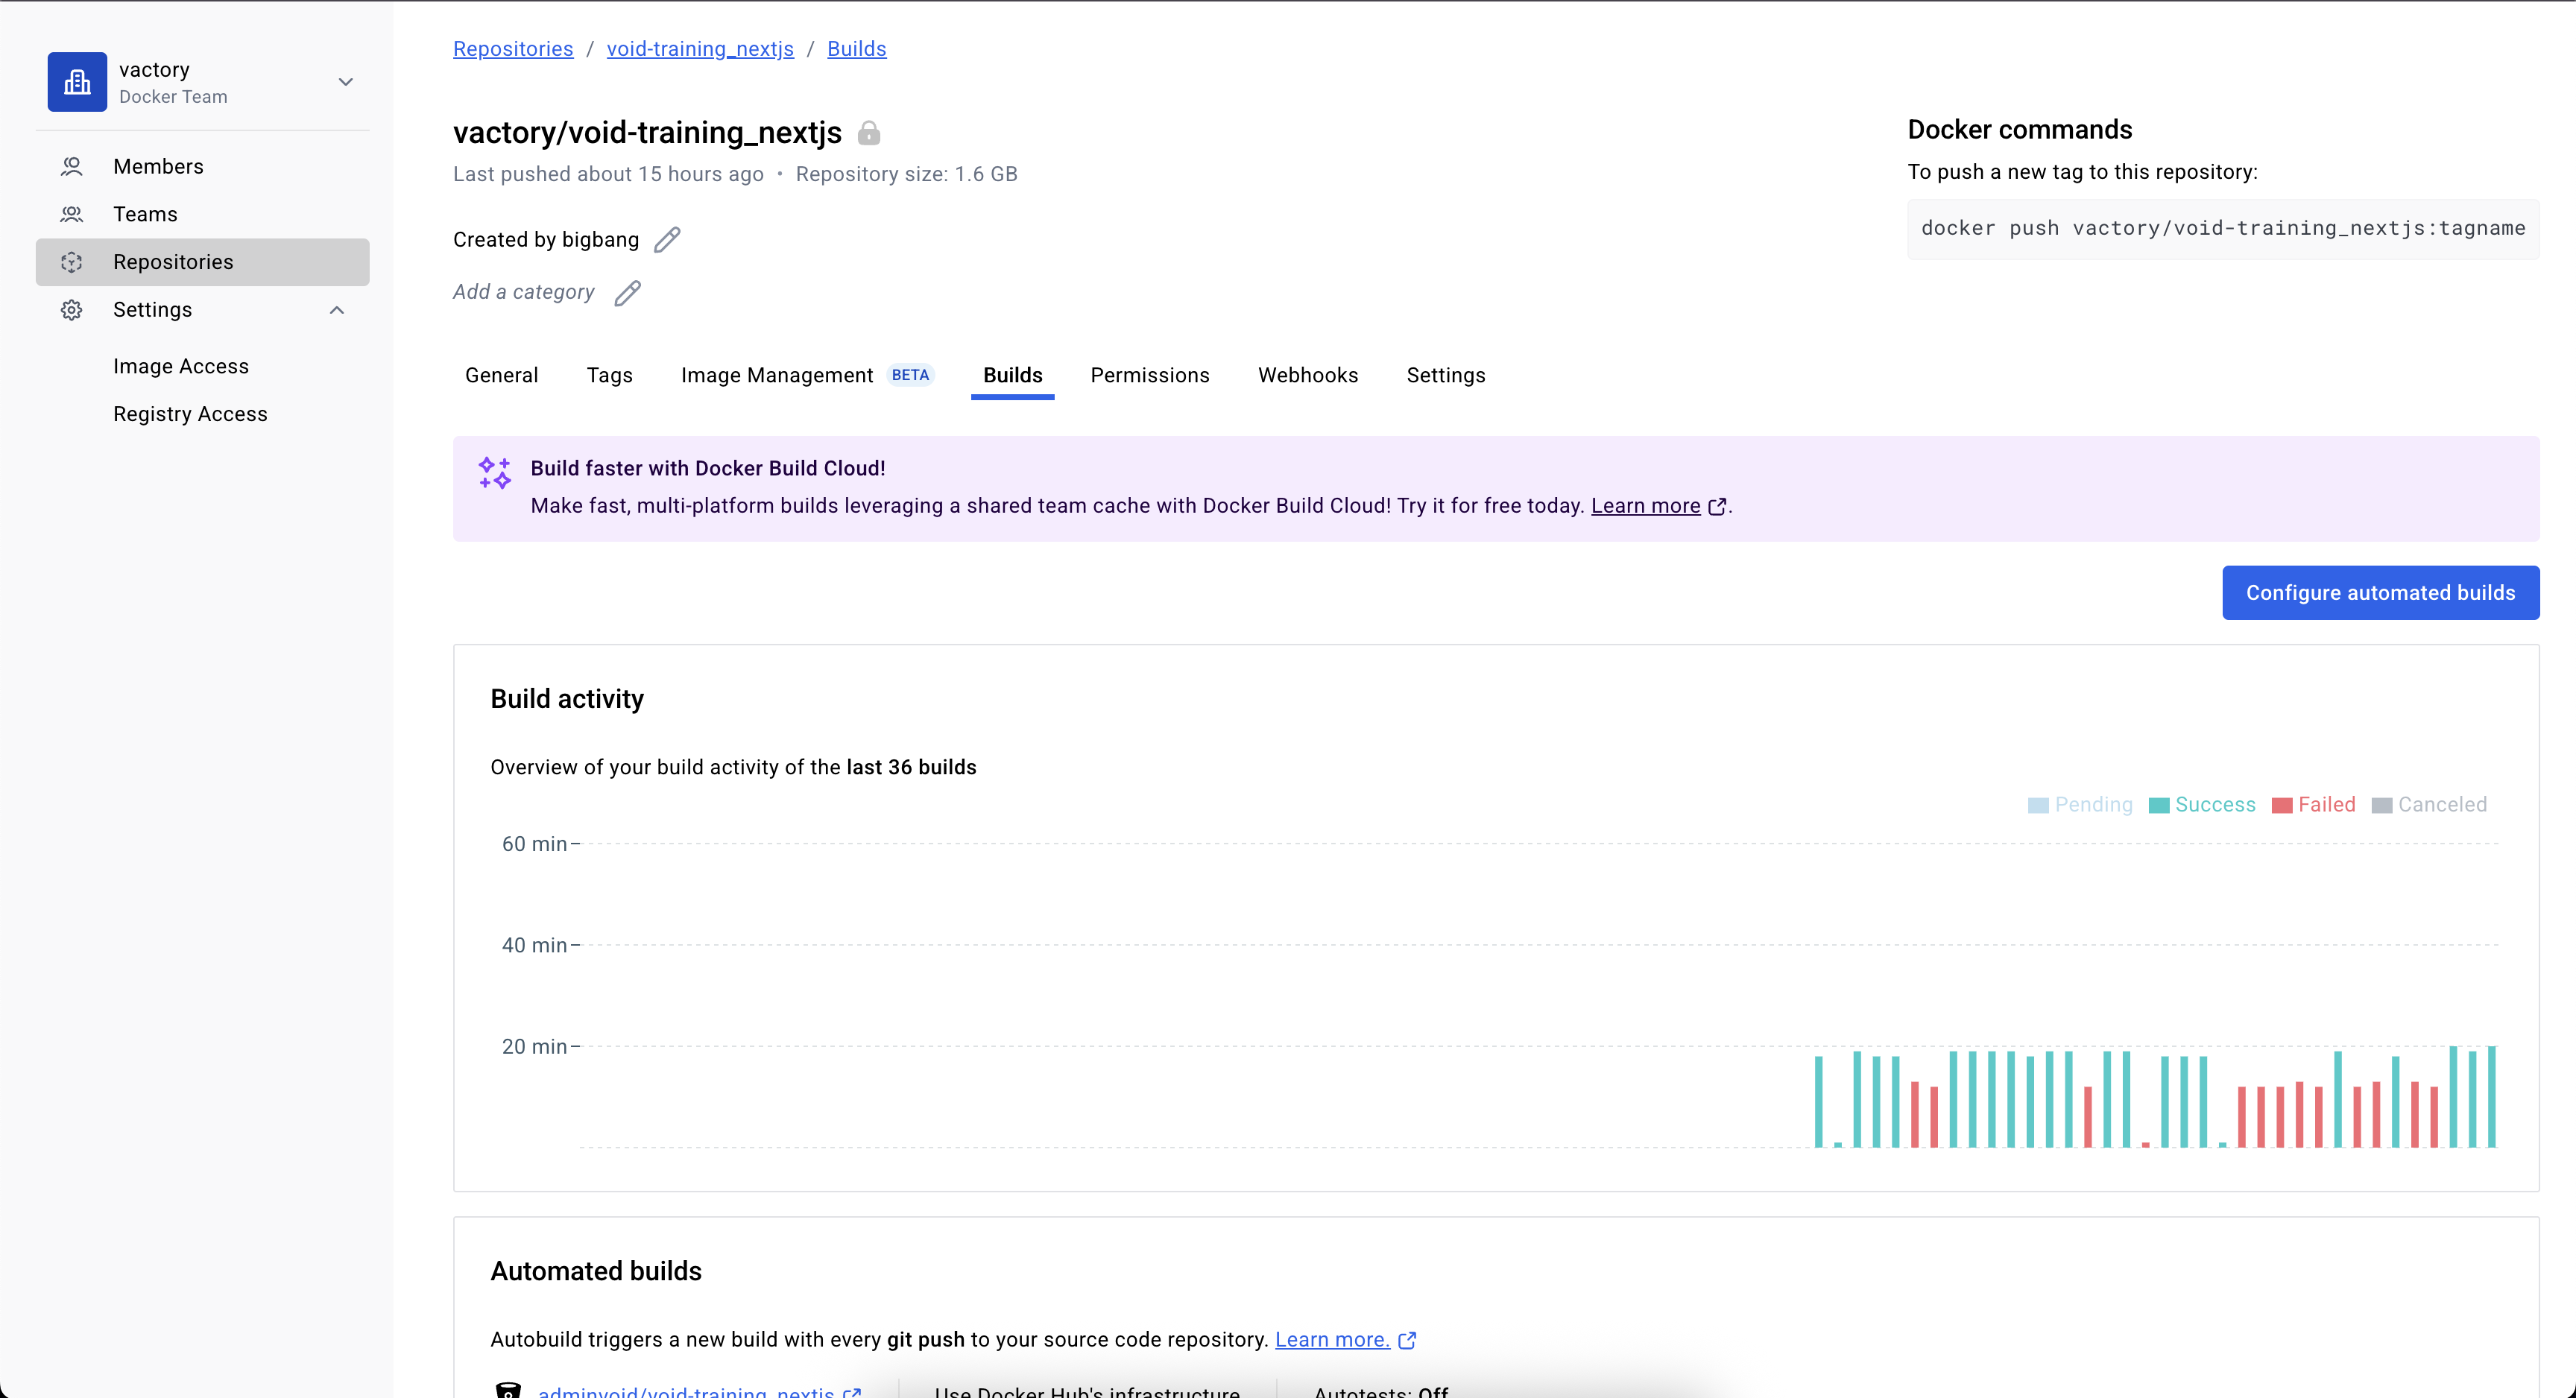
\includegraphics[width=1\textwidth]{images/Screenshot-build.png}
    \caption{DockerHub Frontend Build Process}
    \label{fig:frontend_build}
\end{figure}

% \begin{figure}[H]
%     \centering
%     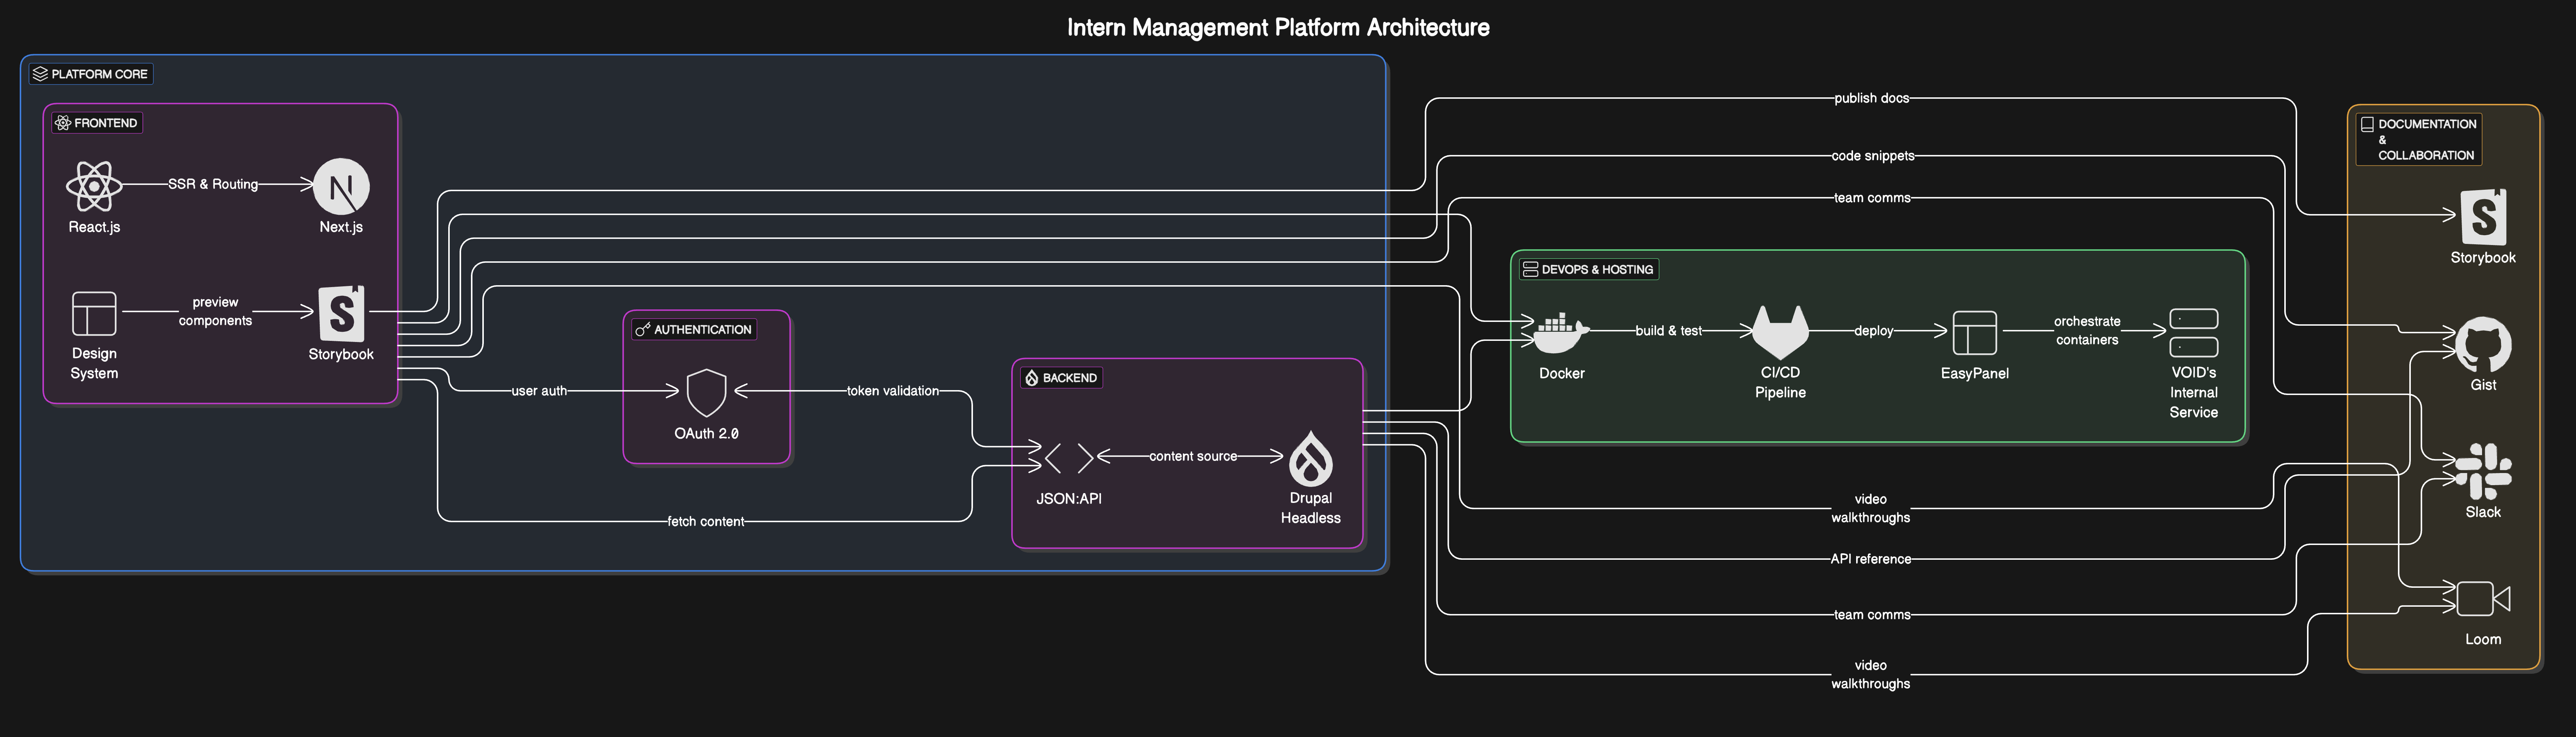
\includegraphics[width=1\textwidth]{images/architecture.png}
%     \caption{DockerHub Build Process}
%     \label{fig:backend_build}
% \end{figure}

\begin{figure}[H]
    \centering
    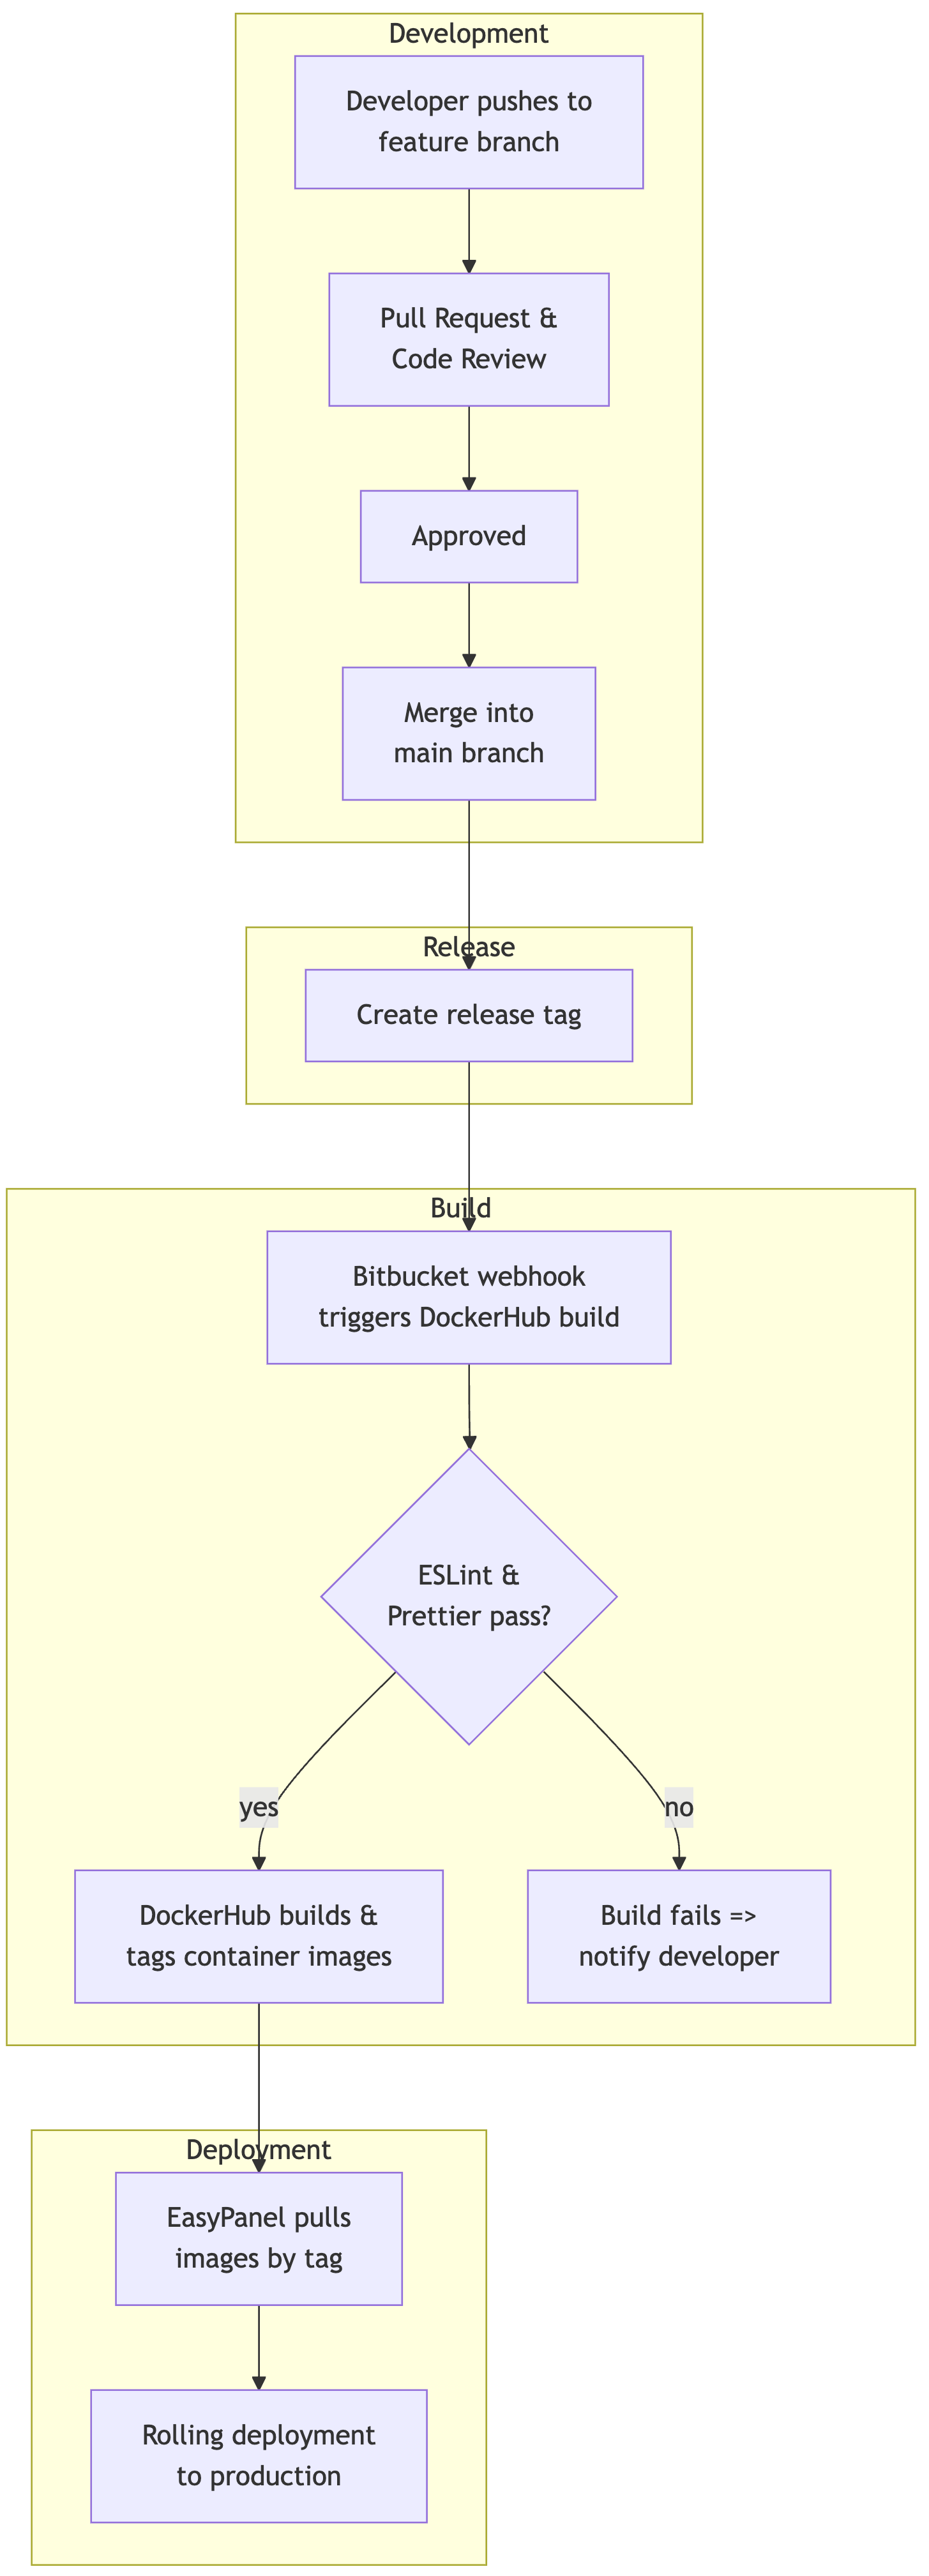
\includegraphics[width=1\textwidth,height=0.9\textheight,keepaspectratio]{images/mermaid-cicd.png}
    \caption{CI/CD Pipeline Overview - Complete workflow from code commit to production deployment}
    \label{fig:cicd_overview}
\end{figure}


% To ensure smooth development, testing, and deployment workflows, a complete CI/CD (Continuous Integration and Continuous Deployment) pipeline was implemented. The main goals were automation, repeatability, and stability in moving from local development to production with minimal manual intervention.

% \subsection{DevOps Stack Overview}

% The stack implemented at \textbf{VOID} is centered around the following tools and services:

% \begin{itemize}
%     \item \textbf{Bitbucket}: Source control system for Git repositories and CI pipeline triggers.
%     \item \textbf{Docker \& Docker Hub} \cite{docker2025multistage}: Used to containerize services and store built images.
%     \item \textbf{EasyPanel}: Lightweight UI-based orchestration platform to manage containers internally on the VOID Mac Studio server.
%     \item \textbf{Drush}: CLI for managing Drupal operations (cache clearing, database import/export, config sync, etc.).
%     \item \textbf{Traefik} \cite{traefik2025docker}: Used as a reverse proxy and load balancer for the application.
% \end{itemize}

% \subsection{CI/CD Workflow Description}

% The CI/CD pipeline was configured to perform the following steps automatically on every push to the \texttt{main} branch:

% \begin{enumerate}
%     \item \textbf{Build Stage:}
%     \begin{itemize}
%         \item Build Docker images for the frontend (Next.js) and backend (Drupal).
%         \item Run unit and integration tests inside the containers.
%     \end{itemize}
%     \item \textbf{Push Stage:}
%     \begin{itemize}
%         \item Push tagged Docker images to the VOID Docker Hub registry.
%     \end{itemize}
%     \item \textbf{Deploy Stage:}
%     \begin{itemize}
%         \item Pull the updated image into the EasyPanel internal server.
%         \item Restart containers via EasyPanel to apply the new version.
%     \end{itemize}
% \end{enumerate}

% \subsection{Bitbucket CI/CD Pipeline Script (Simplified)}

% \begin{verbatim}
% pipelines:
%   branches:
%     main:
%       - step:
%           name: Build and Deploy
%           caches:
%             - docker
%           script:
%             - docker build -t void-candidate-frontend ./frontend
%             - docker build -t void-drupal-backend ./backend
%             - docker push void/void-candidate-frontend
%             - docker push void/void-drupal-backend
% \end{verbatim}

% \subsection{Environment Configuration}

% All environment-specific secrets and settings (API keys, backend URLs, mail server configuration) were injected securely via:

% \begin{itemize}
%     \item Environment variables declared in EasyPanel.
%     \item Bitbucket repository secrets.
%     \item Drupal configuration sync files (\texttt{config/sync/*.yml}).
% \end{itemize}

% \subsection{Automated Dependency Updates}

% A Node.js script was introduced to automate dependency checking and alerting:

% \begin{itemize}
%     \item Scan \texttt{package.json} and \texttt{composer.lock} for outdated dependencies.
%     \item Compare with latest versions from NPM/Packagist.
%     \item Notify the developers via Slack and optionally create a pull request.
% \end{itemize}

% \begin{figure}[H]
%     \centering
%     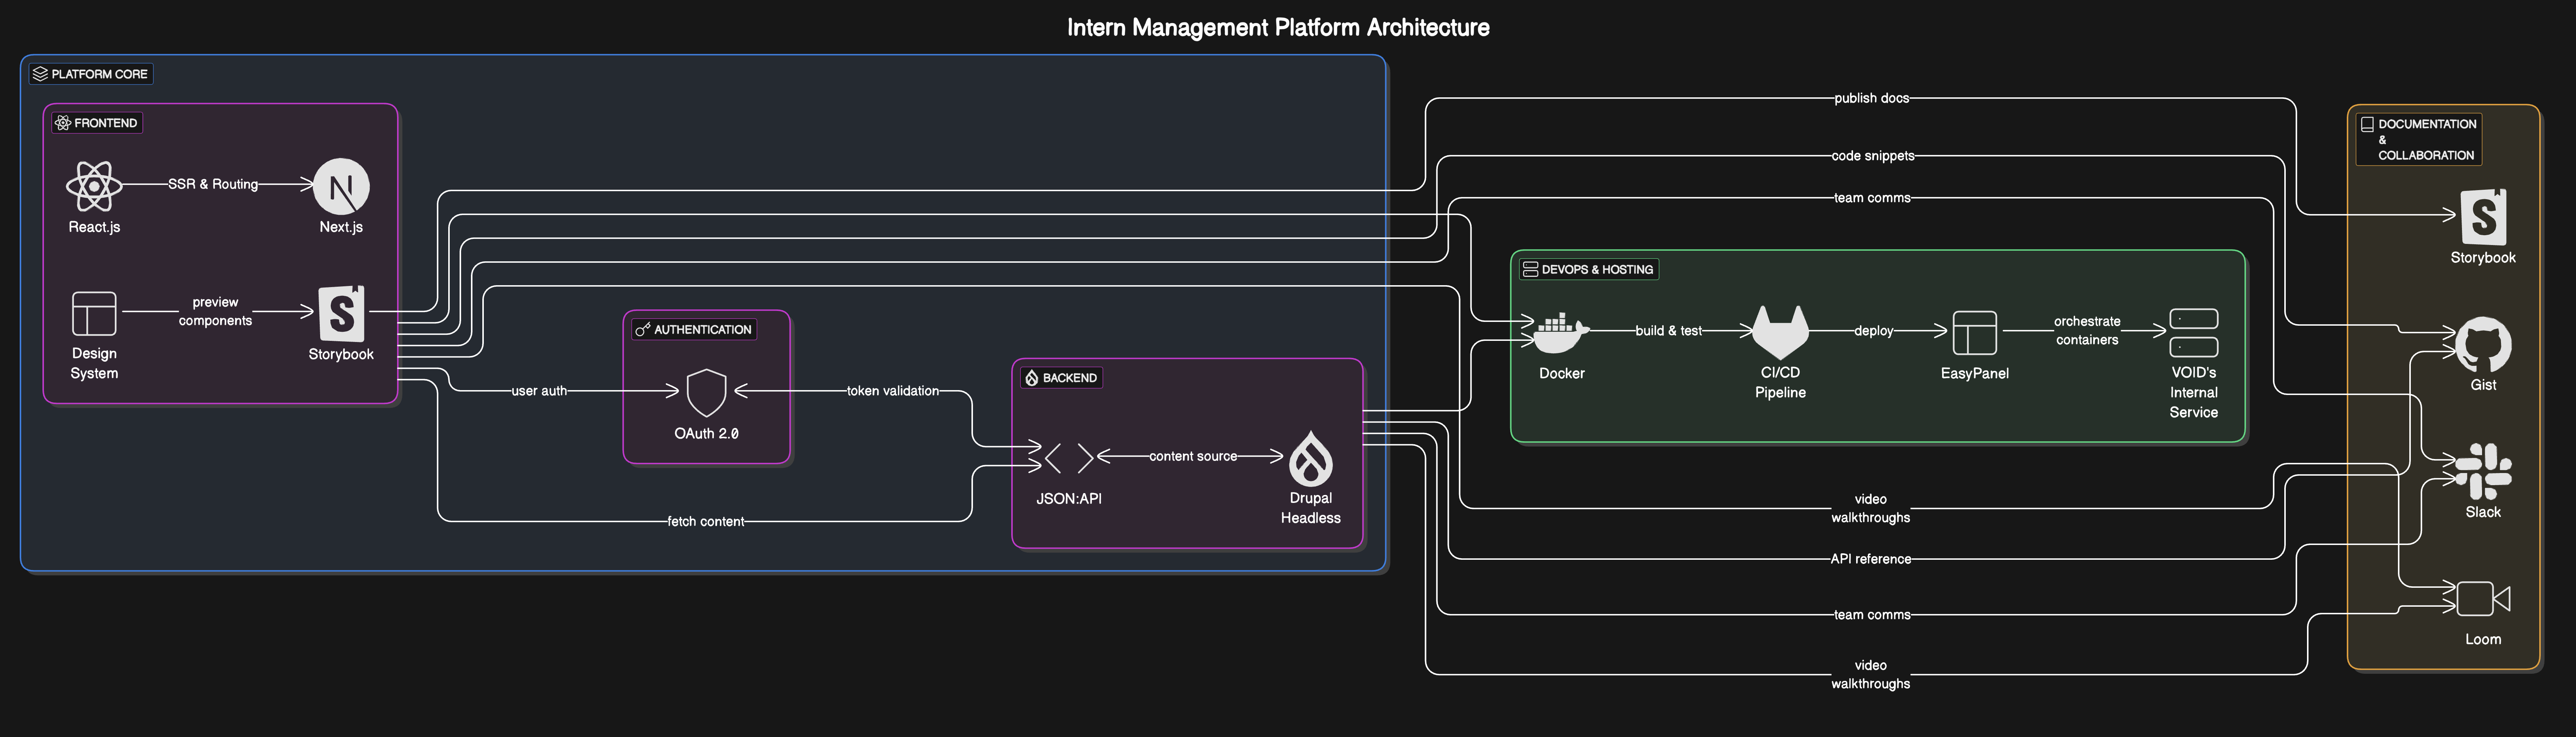
\includegraphics[width=0.95\textwidth]{images/architecture.png}
%     \caption{CI/CD Pipeline for the Intern Management Platform}
%     \label{fig:cicd_pipeline}
% \end{figure}

% \subsection{Benefits Observed}

% The introduction of CI/CD led to the following benefits:

% \begin{itemize}
%     \item \textbf{60\% reduction} in deployment time.
%     \item Elimination of manual production release errors.
%     \item Faster testing feedback and release cycles.
% \end{itemize}

% \bigskip

% \noindent \textit{📌 You should insert a Gantt chart after this section showing the implementation schedule. Let me know if you want one auto-generated in LaTeX or TikZ.}

